% Research paper - IEEE conference format (IEEEtran).
% Build: tectonic paper.tex   (or upload this folder to Overleaf)
% Every number comes from reports/ (see docs/PROJECT_REPORT.md, section 10).
\documentclass[conference]{IEEEtran}
\usepackage[T1]{fontenc}
\usepackage{cite}
\usepackage{amsmath}
\usepackage{newtxtext,newtxmath}  % Times, as in IEEE publications (provides amssymb symbols)
\usepackage{graphicx}
\usepackage{booktabs}
\usepackage{multirow}
\usepackage{xcolor}
\usepackage{tikz}
\usetikzlibrary{arrows.meta,positioning,fit}
\usepackage{url}
\usepackage[hidelinks]{hyperref}

\newcommand{\todo}[1]{\textcolor{red}{[#1]}}

\begin{document}

\title{Human-in-the-Loop Network Intrusion Detection with a Hybrid CNN-LSTM, Uncertainty-Aware Routing and Controlled Retraining}

\author{
\IEEEauthorblockN{\todo{Author 1}, \todo{Author 2}, \todo{Author 3}, \todo{Author 4}}
\IEEEauthorblockA{Department of Computer Engineering\\
\todo{Institute name}, \todo{City}, India\\
\todo{email addresses}}
\and
\IEEEauthorblockN{\todo{Guide name}}
\IEEEauthorblockA{Department of Computer Engineering\\
\todo{Institute name}, \todo{City}, India}
}

\maketitle

\begin{abstract}
Machine-learning intrusion detection systems (IDS) report near-perfect accuracy on benchmark
datasets, yet in operation they fail silently on traffic unlike their training data. We present
an adaptive IDS that treats the security analyst as part of the system. A hybrid CNN-LSTM
classifies network flows; an uncertainty-aware router sends only doubtful flows to an analyst,
using calibrated entropy, a Mahalanobis distance in the network's embedding space, and a Random
Forest ``second opinion''; the analyst's contextual decision is stored in a Knowledge Repository
with similar-incident retrieval; and verified feedback improves the model only through
administrator-approved retraining against acceptance criteria fixed in advance. On the corrected
CIC-IDS2017 dataset, de-duplicated before splitting, every evaluated model exceeds the binary
metrics reported by the reference work (CNN-LSTM F1 99.73\% vs.\ 94.3\%), although tree
ensembles remain slightly more accurate. On a held-out test set of 257,222 flows the deployed
system refers 1.48\% of flows to the analyst, captures 98.9\% of all model errors in that queue,
and is 99.999\% accurate on the flows it handles alone, with two attacks auto-closed and no false
alerts. Leave-one-attack-out experiments show that the CNN-LSTM alone is confidently wrong on
unseen attacks (up to 97\% missed), while the hybrid router misses at most 10.2\% in five of six
unseen attack types; SSH brute force remains undetected by all methods.
\end{abstract}

\begin{IEEEkeywords}
intrusion detection, human-in-the-loop, uncertainty estimation, CNN-LSTM, out-of-distribution detection, CIC-IDS2017, selective classification
\end{IEEEkeywords}

%=====================================================================
\section{Introduction}
Network intrusion detection is a long-standing application of machine learning, and deep models
such as hybrid convolutional-recurrent networks now report accuracies above 98\% on public
benchmarks. Such figures overstate operational readiness for three reasons. First, benchmark
datasets contain labelling errors and duplicated flows that inflate test scores
\cite{engelen2021troubleshooting,liu2022error}. Second, identifier-like features (addresses,
ports, timestamps) allow models to learn shortcuts rather than attack behaviour
\cite{arp2022dos}. Third, and most importantly, a classifier deployed in a real network will meet
attacks it has never seen, and a standard softmax classifier has no way to say ``I don't
know'' \cite{sommer2010outside,hendrycks2017baseline}.

A recent study \cite{refpaper2025} proposed an uncertainty-aware adaptive IDS combining a hybrid
CNN-LSTM classifier, cWGAN-GP data augmentation and human-in-the-loop feedback, reporting 98\%
binary accuracy, 96.6\% detection rate, 92.1\% precision and 94.3\% F1. We re-implement its
classifier and extend the idea into a complete, working system whose central question is not
``how accurate is the model?'' but ``which flows can be trusted to the model, and which must a
human see?''

Our contributions are:
\begin{enumerate}
\item A leakage-controlled evaluation of the reference CNN-LSTM, Random Forest and LightGBM on the
corrected CIC-IDS2017 dataset, with shortcut features removed and de-duplication performed before
splitting, over three random seeds, including LSTM and augmentation ablations.
\item Evidence from leave-one-attack-out and day-based experiments that the CNN-LSTM's own
uncertainty misses most unseen attacks, and a hybrid routing rule (entropy, embedding distance
and a Random Forest second opinion) that routes them to an analyst.
\item An end-to-end human-in-the-loop platform: traffic replay, analyst console with contextual
feedback, a Knowledge Repository with similar-incident retrieval, and controlled retraining with
pre-registered acceptance criteria, administrator approval, deployment and rollback.
\end{enumerate}

%=====================================================================
\section{Related Work}
\textit{Datasets.} CIC-IDS2017 \cite{sharafaldin2018toward} is among the most used flow-based IDS
benchmarks. Engelen \textit{et al.}\ \cite{engelen2021troubleshooting} and Liu \textit{et al.}\
\cite{liu2022error} documented flow-construction and labelling errors in it and released a
corrected version, which we use.

\textit{Deep and classical models.} Recurrent networks \cite{hochreiter1997lstm} and hybrid
CNN-LSTM architectures \cite{refpaper2025} learn from ordered feature vectors, while tree
ensembles such as Random Forest \cite{breiman2001random} and LightGBM \cite{ke2017lightgbm} remain
strong baselines on tabular flow features.

\textit{Pitfalls.} Arp \textit{et al.}\ \cite{arp2022dos} catalogue common errors in ML for
security, including data snooping, spurious correlations and inappropriate baselines; Sommer and
Paxson \cite{sommer2010outside} argue that intrusion detection is closer to anomaly detection in
an open world than to closed-set classification.

\textit{Uncertainty.} Temperature scaling \cite{guo2017calibration} calibrates softmax outputs;
maximum-softmax and entropy scores detect misclassified inputs \cite{hendrycks2017baseline};
class-conditional Mahalanobis distance in feature space detects out-of-distribution inputs
\cite{lee2018simple}; ensembles give better uncertainty than single networks
\cite{lakshminarayanan2017simple}. Selective classification \cite{geifman2017selective} formalises
the trade-off between coverage and risk that underlies referral to a human.

\textit{Augmentation.} Conditional GANs \cite{mirza2014conditional} trained with the Wasserstein
gradient-penalty objective \cite{gulrajani2017improved} (cWGAN-GP) are used to synthesise
minority-class traffic \cite{refpaper2025}.

%=====================================================================
\section{Dataset and Preprocessing}
We use the corrected CIC-IDS2017 release \cite{engelen2021troubleshooting,liu2022error}: five
daily capture files (Monday--Friday) totalling 2,099,976 flows with 91 columns and 27 labels.
An exploratory analysis found no missing values, five flows with infinite rate features, no exact
duplicate rows, but 12.5\% duplicates once identifier columns are ignored.

\textit{Feature hygiene.} We drop flow ID, source and destination IP, source port, timestamp and
row identifier, since they identify hosts rather than behaviour. The corrected release's
``Attempted Category'' column is also dropped because it encodes the label. Destination port is
excluded as a shortcut feature (in this dataset, port 21 almost uniquely identifies FTP-Patator).

\textit{Label mapping.} Unsuccessful ``Attempted'' attacks are merged into their attack class;
\textit{Infiltration--Portscan} is merged into \textit{Portscan} (identical features); the three
web attacks (brute force, XSS, SQL injection) are grouped. This yields 13 classes. Heartbleed
(11 flows) and Infiltration (81 flows) are too small for reliable per-class estimates; we report
macro-F1 both with and without them (``reliable'').

\textit{De-duplication before splitting.} Rows identical in all model-visible features and label
are collapsed (385,106 rows), and 58 rows whose features appear with two different labels are
removed. Removing destination port revealed that most Portscan rows were copies of one another
(230,833 $\rightarrow$ 7,695). The remaining 1,714,812 flows are split 70/15/15, stratified by
class (Table~\ref{tab:classes}); a hash check confirms no feature vector appears in two splits.

\textit{Transform.} Fitted on the training split only: infinite values and NaN are replaced by
the training median; a signed logarithm $\mathrm{sign}(x)\log(1+|x|)$ compresses heavy-tailed
features; one constant and 17 near-duplicate features ($|\rho|>0.99$) are removed, leaving 64;
features are standardised. The fitted transform, feature order and label map are saved with each
model so that training and deployment apply identical transformations.

\begin{table}[t]
\caption{Flows per class after mapping and de-duplication}
\label{tab:classes}
\centering
\footnotesize
\begin{tabular}{lrrr}
\toprule
Class & Train & Validation & Test \\
\midrule
BENIGN & 996,410 & 213,517 & 213,516 \\
DoS Hulk & 111,333 & 23,857 & 23,858 \\
DDoS & 66,601 & 14,272 & 14,271 \\
Portscan & 5,386 & 1,154 & 1,155 \\
DoS GoldenEye & 5,353 & 1,147 & 1,147 \\
DoS Slowloris & 3,992 & 855 & 856 \\
DoS Slowhttptest & 3,576 & 766 & 766 \\
FTP-Patator & 2,789 & 597 & 598 \\
SSH-Patator & 2,092 & 448 & 448 \\
Web Attack & 1,439 & 309 & 308 \\
Botnet & 1,343 & 288 & 288 \\
Infiltration$^\dagger$ & 46 & 10 & 10 \\
Heartbleed$^\dagger$ & 8 & 2 & 1 \\
\midrule
Total & 1,200,368 & 257,222 & 257,222 \\
\bottomrule
\multicolumn{4}{l}{$^\dagger$Too few samples for reliable per-class metrics.}
\end{tabular}
\end{table}

%=====================================================================
\section{Methodology}

\begin{figure*}[t]
\centering
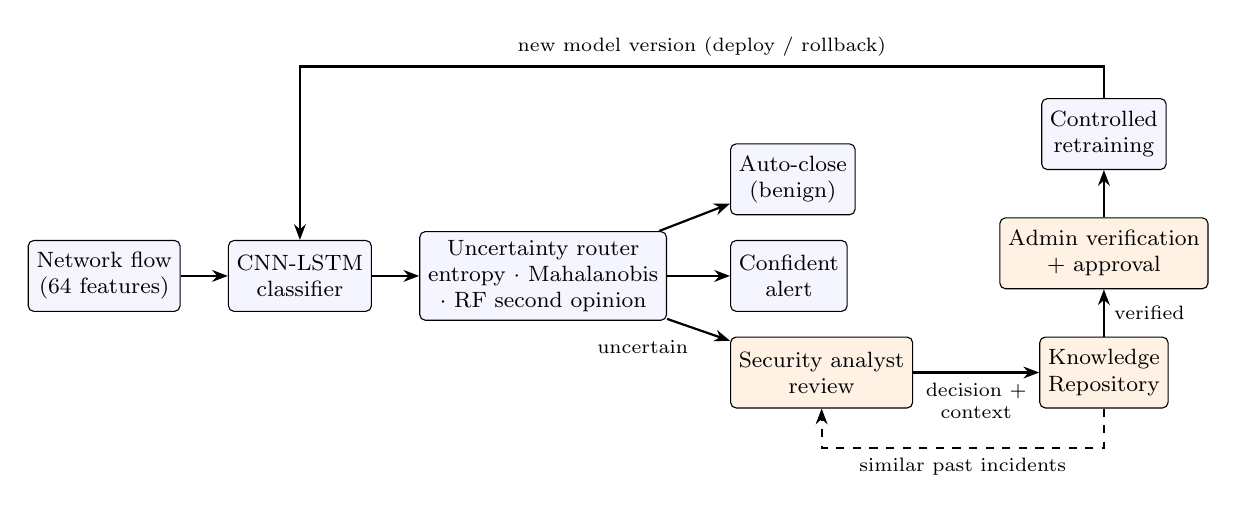
\begin{tikzpicture}[
  box/.style={draw, rounded corners=2pt, align=center, font=\footnotesize, minimum height=9mm, inner sep=3pt, fill=blue!4},
  hum/.style={box, fill=orange!10},
  arr/.style={-{Stealth[length=2mm]}, thick},
  lab/.style={font=\scriptsize, align=center}]
\node[box] (flow) {Network flow\\(64 features)};
\node[box, right=6mm of flow] (cnn) {CNN-LSTM\\classifier};
\node[box, right=6mm of cnn] (unc) {Uncertainty router\\entropy $\cdot$ Mahalanobis\\$\cdot$ RF second opinion};
\node[box, above right=2mm and 8mm of unc] (benign) {Auto-close\\(benign)};
\node[box, right=8mm of unc] (alert) {Confident\\alert};
\node[hum, below right=2mm and 8mm of unc] (analyst) {Security analyst\\review};
\node[hum, right=16mm of analyst] (kr) {Knowledge\\Repository};
\node[hum, above=6mm of kr] (admin) {Admin verification\\+ approval};
\node[box, above=6mm of admin] (retrain) {Controlled\\retraining};
\draw[arr] (flow) -- (cnn);
\draw[arr] (cnn) -- (unc);
\draw[arr] (unc) -- (benign);
\draw[arr] (unc) -- (alert);
\draw[arr] (unc) -- node[lab, below left]{uncertain} (analyst);
\draw[arr] (analyst) -- node[lab, below]{decision +\\context} (kr);
\draw[arr] (kr) -- node[lab, right]{verified} (admin);
\draw[arr] (admin) -- (retrain);
\draw[arr] (retrain.north) |- ++(0,4mm) -| node[lab, above, pos=0.25]{new model version (deploy / rollback)} (cnn.north);
\draw[arr, dashed] (kr.south) |- ++(0,-5mm) -| node[lab, below, pos=0.25]{similar past incidents} (analyst.south);
\end{tikzpicture}
\caption{System overview. Only uncertain flows reach the analyst; verified analyst decisions
improve the model only through administrator-approved retraining.}
\label{fig:system}
\end{figure*}

\subsection{Classifier}
Following the reference architecture \cite{refpaper2025}, the 64-feature vector is treated as a
one-channel sequence: Conv1D(64, kernel 5, ReLU) $\rightarrow$ MaxPool(2) $\rightarrow$
Conv1D(128, kernel 3, ReLU) $\rightarrow$ LSTM(128) $\rightarrow$ Dropout(0.3) $\rightarrow$
Dense(13). The final LSTM state $\mathbf{z}\in\mathbb{R}^{128}$ is the flow's embedding. The
network is trained with plain cross-entropy (AdamW, learning rate $10^{-3}$, batch 1024, cosine
schedule, at most 20 epochs, early stopping on validation macro-F1). Unweighted loss keeps
probabilities calibratable; instead, classes with fewer than 1,000 training rows are randomly
oversampled in the training split only. Without this the network never predicts Heartbleed or
Infiltration and validation macro-F1 is capped near 0.85.

\subsection{Baselines and ablations}
Random Forest (100 trees) and LightGBM (early stopping on validation; leaf outputs capped because
unconstrained training diverged after 12 rounds) are trained on the identical transformed
features. Ablations remove the LSTM (global average pooling of the convolutional features),
add cWGAN-GP augmentation, and remove calibration.

\subsection{Minority augmentation}
A conditional WGAN-GP \cite{mirza2014conditional,gulrajani2017improved} (two 256-unit layers per
network, gradient penalty $\lambda=10$, five critic steps per generator step) is trained on
training rows of classes with 100--5,000 examples and generates samples up to 5,000 per class.
A synthetic sample is kept only if the baseline Random Forest assigns it to its conditioning
class. Unlike the reference work we sample from Gaussian noise rather than VAE-encoded seeds.

\subsection{Calibration and uncertainty signals}
The validation split is divided into a calibration half and an evaluation half. On the
calibration half we fit a temperature $T$ \cite{guo2017calibration} and compute, for each flow,
\begin{equation}
H(\mathbf{x}) = -\frac{1}{\log K}\sum_{k=1}^{K} p_k \log p_k, \quad
\mathbf{p} = \mathrm{softmax}(\mathbf{f}(\mathbf{x})/T),
\end{equation}
the normalised entropy over $K=13$ classes, and the class-conditional Mahalanobis distance
\cite{lee2018simple}
\begin{equation}
D(\mathbf{x}) = \min_{c} (\mathbf{z}-\boldsymbol{\mu}_c)^\top \boldsymbol{\Sigma}^{-1} (\mathbf{z}-\boldsymbol{\mu}_c),
\end{equation}
with class means $\boldsymbol{\mu}_c$ and a shared, shrunk covariance $\boldsymbol{\Sigma}$
estimated on training embeddings. Thresholds are quantiles on the calibration half: $\tau_H$ at
the 99th percentile of $H$ and $\tau_D$ at the 99.5th percentile of $D$.

\subsection{Hybrid routing}
A flow is \emph{uncertain} if
\begin{equation}
H>\tau_H \;\lor\; D>\tau_D \;\lor\; u_{\mathrm{RF}}>\tau_{\mathrm{RF}} \;\lor\; \hat{y}_{\mathrm{RF}}\neq\hat{y},
\end{equation}
and each flow receives one of three decisions:
\begin{equation}
\text{decision}(\mathbf{x}) =
\begin{cases}
\text{review} & \text{if uncertain},\\
\text{auto-alert} & \text{else if } \hat{y}\neq\text{BENIGN},\\
\text{auto-benign} & \text{otherwise,}
\end{cases}
\end{equation}
where $\hat{y}$ is the CNN-LSTM prediction, $\hat{y}_{\mathrm{RF}}$ the Random Forest prediction,
$u_{\mathrm{RF}} = 1-\max_k p^{\mathrm{RF}}_k$ its vote-spread uncertainty and $\tau_{\mathrm{RF}}$ its
99.5th percentile on the calibration half. The Random Forest terms were added after the
leave-one-attack-out experiment (Section~\ref{sec:loao}) showed that the CNN-LSTM's own signals
miss most unseen attacks; we state this explicitly because it means that experiment is not an
independent test of the hybrid rule, whereas the untouched test set is.

\subsection{Human-in-the-loop platform}
The platform (Fig.~\ref{fig:system}) consists of a FastAPI service with an SQLite store and a
React web client with three sections (About, Analyst, Administration).
\begin{itemize}
\item \textit{Traffic replay} streams the untouched test split through the deployed model. Each
flow's true label is stored only for the administrator's evaluation panel; it is never used for
prediction or shown to analysts, which an automated test verifies.
\item \textit{Analyst console}: for each referred flow the analyst sees network context (addresses,
ports, time), class probabilities, the second opinion, the uncertainty values against their
thresholds, the most atypical features, and similar past incidents. The analyst records a
verdict, class, reason, context, evidence, confidence, comments and tags.
\item \textit{Knowledge Repository}: every decision becomes a searchable incident. Similar
incidents are retrieved by cosine similarity of CNN-LSTM embeddings, recomputed whenever the
deployed model changes because embeddings from different model versions are not comparable.
\item \textit{Controlled retraining}: only administrator-verified decisions are used. A candidate
is fine-tuned from the deployed model on the verified feedback (70\%) plus a 200,000-row
stratified sample of the original training data (to prevent forgetting), recalibrated, and
evaluated against the deployed model on a fixed benchmark (the validation evaluation half) and on
the held-out feedback (30\%). Acceptance criteria, fixed in configuration and copied into the job
when it is created, require a macro-F1 drop of at most 0.5 points, a false-positive-rate increase
of at most 0.05 points, and no loss of accuracy on held-out feedback. A passing candidate still
requires administrator approval before deployment; deployment and rollback swap models without
restarting the service, and every action is written to an audit log.
\end{itemize}

%=====================================================================
\section{Experimental Setup}
All models are trained on the training split and selected on the validation split. The test split
was used exactly once, after all design decisions, including the hybrid rule, were fixed. Results
are the mean $\pm$ standard deviation over seeds 42, 7 and 2025; the deployed system uses the
seed-42 CNN-LSTM and Random Forest. Accuracy is 13-class accuracy; precision, detection rate
(recall), F1, false-positive rate (FPR) and false-negative rate treat all attacks as one positive
class, matching the reference work. Experiments ran on an Intel Core i5-1240P with 7.7\,GB RAM and
an NVIDIA RTX 2050 (4\,GB) using PyTorch \cite{paszke2019pytorch} and scikit-learn
\cite{pedregosa2011scikit}.

\textit{Generalisation experiments.} (i) Leave-one-attack-out: for each of six attacks, all its
rows are removed from training and calibration, the whole pipeline (CNN-LSTM for 8 epochs,
calibration, thresholds, Random Forest) is refitted with one seed, and we measure how the unseen
attack's flows (training and validation rows) are routed. (ii) Day-based split: train on
Monday--Wednesday, evaluate on Thursday--Friday, where every attack type is new. Both use
non-test rows only.

%=====================================================================
\section{Results}

\subsection{Classification on the held-out test set}
Table~\ref{tab:main} compares all models with the numbers reported by the reference work.
Every model, including our re-implementation of the CNN-LSTM, exceeds the reported binary
metrics. The comparison is not like-for-like: we use the corrected dataset, remove duplicates
before splitting and exclude shortcut features, and differences in preprocessing are known to
change results substantially \cite{engelen2021troubleshooting,arp2022dos}. Tree ensembles are the
most accurate models: the Random Forest reaches 99.23\% reliable macro-F1 against 98.09\% for the
CNN-LSTM, with a lower false-positive rate (0.020\% vs.\ 0.059\%).

\begin{table*}[t]
\caption{Held-out test set (257,222 flows), mean $\pm$ standard deviation over three seeds (\%)}
\label{tab:main}
\centering
\footnotesize
\begin{tabular}{lcccccc}
\toprule
Metric & Reported \cite{refpaper2025} & Random Forest & LightGBM & CNN-LSTM & CNN-LSTM + aug. & CNN (no LSTM) \\
\midrule
Accuracy & 98.0$^\ast$ & \textbf{99.97} $\pm$ 0.00 & 99.96 $\pm$ 0.00 & 99.89 $\pm$ 0.07 & 99.92 $\pm$ 0.02 & 99.80 $\pm$ 0.02 \\
Detection rate & 96.6 & \textbf{99.92} $\pm$ 0.00 & 99.91 $\pm$ 0.01 & 99.75 $\pm$ 0.24 & 99.86 $\pm$ 0.05 & 99.23 $\pm$ 0.10 \\
Precision & 92.1 & \textbf{99.90} $\pm$ 0.00 & 99.84 $\pm$ 0.01 & 99.71 $\pm$ 0.07 & 99.74 $\pm$ 0.03 & 99.70 $\pm$ 0.01 \\
F1 & 94.3 & \textbf{99.91} $\pm$ 0.00 & 99.88 $\pm$ 0.01 & 99.73 $\pm$ 0.16 & 99.80 $\pm$ 0.04 & 99.46 $\pm$ 0.05 \\
Macro-F1 (13 classes) & -- & \textbf{99.07} $\pm$ 0.22 & 98.32 $\pm$ 0.04 & 96.71 $\pm$ 3.06 & 97.46 $\pm$ 1.36 & 94.12 $\pm$ 1.42 \\
Macro-F1 (reliable) & -- & \textbf{99.23} $\pm$ 0.02 & 99.03 $\pm$ 0.05 & 98.09 $\pm$ 0.99 & 98.47 $\pm$ 0.25 & 96.39 $\pm$ 0.32 \\
FPR & -- & \textbf{0.020} $\pm$ 0.000 & 0.033 $\pm$ 0.003 & 0.059 $\pm$ 0.015 & 0.054 $\pm$ 0.005 & 0.062 $\pm$ 0.002 \\
\bottomrule
\multicolumn{7}{l}{$^\ast$Binary accuracy in \cite{refpaper2025}; ours is 13-class accuracy. ``Reliable'' excludes Heartbleed and Infiltration.}
\end{tabular}
\end{table*}

\begin{table}[t]
\caption{Per-class recall on the test set (\%, mean over three seeds)}
\label{tab:perclass}
\centering
\footnotesize
\begin{tabular}{lccc}
\toprule
Class & RF & LightGBM & CNN-LSTM \\
\midrule
BENIGN & 99.98 & 99.97 & 99.94 \\
DoS Hulk & 100.00 & 99.99 & 99.90 \\
DDoS & 100.00 & 100.00 & 99.99 \\
Portscan & 99.65 & 99.65 & 96.65 \\
DoS GoldenEye & 100.00 & 99.91 & 98.23 \\
DoS Slowloris & 100.00 & 100.00 & 99.10 \\
DoS Slowhttptest & 98.87 & 99.09 & 98.96 \\
FTP-Patator & 100.00 & 100.00 & 99.78 \\
SSH-Patator & 99.70 & 99.70 & 99.48 \\
Web Attack & 97.94 & 98.38 & 96.54 \\
Botnet & 94.79 & 92.01 & 89.35 \\
Infiltration$^\dagger$ & 93.33 & 80.00 & 93.33 \\
Heartbleed$^\dagger$ & 100.00 & 100.00 & 100.00 \\
\bottomrule
\multicolumn{4}{l}{$^\dagger$10 and 1 test flows respectively.}
\end{tabular}
\end{table}

Per-class recall (Table~\ref{tab:perclass}) shows that the CNN-LSTM's deficit concentrates in
Portscan, Botnet and Web Attack. Botnet is the hardest reliable class for every model.

\subsection{Ablations}
Removing the LSTM lowers reliable macro-F1 by 1.7 points and Portscan recall from 96.7\% to
88.8\%, supporting the hybrid convolutional-recurrent design. Augmentation raises mean reliable
macro-F1 by 0.4 points and reduces its variance across seeds (standard deviation 0.99 $\rightarrow$
0.25), but the gain is within seed-to-seed variation. The synthetic samples are trivially
separable from real ones (a real-versus-synthetic classifier reaches AUC 1.0 for all six augmented
classes), because real flow features are discrete counts while the generator outputs continuous
values. Temperature scaling found $T=1.01$: the CNN-LSTM was already well calibrated (expected
calibration error 0.023\% before and 0.022\% after), so removing calibration has no measurable
effect in our setting.

\subsection{Routing on the test set}
Table~\ref{tab:routing} reports the deployed system. It sends 1.48\% of flows to the analyst,
and 98.9\% of all CNN-LSTM errors fall inside that queue, so the accuracy on the 98.5\% of
flows handled automatically is 99.999\%. Of 43,706 attack flows, two were auto-closed as benign;
no benign flow was raised as a confident alert. Compared with routing on the CNN-LSTM's own
signals, the second opinion costs 0.15 points of additional referral and reduces missed attacks
from seven to two. Referral is concentrated where the classifier is weakest: all Infiltration and 99.7\% of Web
Attack flows, 75\% of DoS Slowhttptest, 63\% of Botnet and 38\% of Portscan are reviewed,
against under 1\% of BENIGN, DDoS and DoS Hulk flows.

\begin{table}[t]
\caption{Deployed routing on the test set}
\label{tab:routing}
\centering
\footnotesize
\begin{tabular}{lcc}
\toprule
 & Hybrid & CNN-LSTM \\
 & (deployed) & signals only \\
\midrule
Referred to analyst & 1.48\% & 1.33\% \\
Accuracy, auto-handled & \textbf{99.999\%} & 99.997\% \\
Errors caught by review & \textbf{98.9\%} & 96.0\% \\
Attacks auto-closed & \textbf{2} & 7 \\
Benign auto-alerted & 0 & 0 \\
\bottomrule
\end{tabular}
\end{table}

\subsection{Unseen attacks: leave-one-attack-out}
\label{sec:loao}
Fig.~\ref{fig:loao} shows the share of each unseen attack's flows that were auto-closed as benign.
In a first run, the CNN-LSTM's own signals missed 80.5\% of unseen Portscan and 32.9\% of unseen
Botnet, while a Random Forest using only its vote spread missed 5.3\% and 10.8\%. In the rerun
shown, the CNN-LSTM missed 97.0\% of unseen web attacks (13.1\% in the first run), revealing high
run-to-run variance in how the network behaves on data it has not seen. The hybrid rule missed
the fewest unseen flows for five of six attacks (at most 10.2\%) at a normal-traffic referral of
about 1.4\%, against 0.55\% for the Random Forest alone. SSH brute force was missed by every method:
individually, its flows are indistinguishable from legitimate SSH sessions.

\begin{figure}[t]
\centering
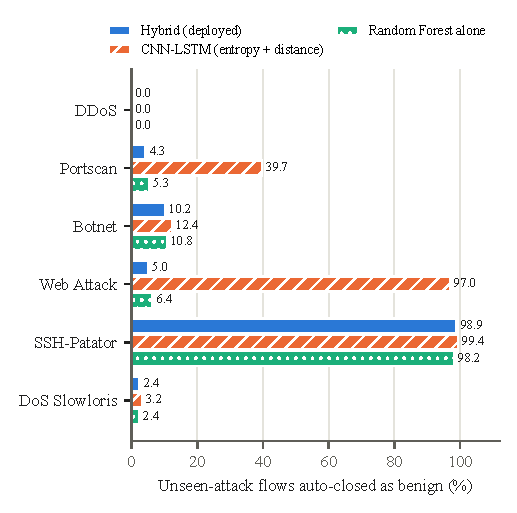
\includegraphics[width=\columnwidth]{figs/loao_missed.pdf}
\caption{Leave-one-attack-out: share of the held-out attack's flows auto-closed as benign
(lower is better). Each group retrains the full pipeline without that attack.}
\label{fig:loao}
\end{figure}

\subsection{Unseen days}
Trained on Monday--Wednesday and evaluated on Thursday--Friday, the hybrid rule auto-closed 1.38\%
of attack flows, compared with 16.46\% for the CNN-LSTM's entropy and distance and 35.28\% for
entropy alone; the Mahalanobis distance therefore halves the CNN-LSTM's misses, but the second
opinion is needed to close the gap. The Random Forest alone missed 1.45\%. The hybrid referred
0.76\% of benign flows (Random Forest: 0.50\%). Per class (Fig.~\ref{fig:day}), Botnet remains
difficult (37.7\% missed).

\begin{figure}[t]
\centering
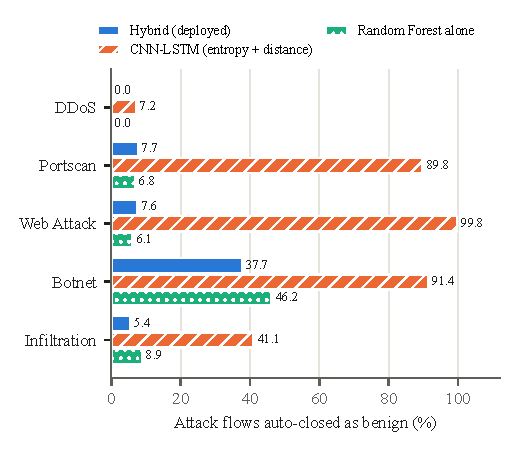
\includegraphics[width=\columnwidth]{figs/day_missed.pdf}
\caption{Day-based split (train Monday--Wednesday, evaluate Thursday--Friday): share of each
unseen attack class auto-closed as benign.}
\label{fig:day}
\end{figure}

\subsection{System behaviour}
During replay the service scores a flow in about 0.55\,ms on the CPU, including the second
opinion. An automated end-to-end scenario test exercises replay, analyst feedback, Knowledge
Repository retrieval, administrator verification, retraining, acceptance checks, approval,
deployment, rollback and audit logging, and asserts that true labels never reach analyst
endpoints.

%=====================================================================
\section{Discussion}
\textit{Accuracy is not the bottleneck.} Once leakage is controlled, all models exceed 99.7\% binary
F1 on a random split, and tree ensembles are marginally better than the CNN-LSTM. What
distinguishes systems is how they behave on traffic unlike their training data, which a random
split does not measure.

\textit{A confident network is not a safe network.} The CNN-LSTM's own uncertainty signals missed
up to 97\% of an unseen attack, and its behaviour on unseen attacks varied strongly between runs.
Combining it with a structurally different model and referring disagreements to a human was the
single most effective change we made; this agrees with the broader finding that ensembles give
more reliable uncertainty than single networks \cite{lakshminarayanan2017simple}.

\textit{Threats to validity.} The hybrid rule was designed after observing the
leave-one-attack-out results, so those results favour it; the test set, used once, is the
independent check, but it contains no unseen attack types. Leave-one-attack-out used one seed per
attack. The comparison with the reference work mixes datasets and preprocessing. Classes with fewer
than 100 samples cannot be evaluated reliably. The analyst workflow was exercised by the authors,
not by practising security analysts.

\textit{Limitations.} Per-flow models cannot see attacks defined by many flows, such as SSH brute
force and parts of Botnet traffic; host- and time-window features are needed. The Random Forest
second opinion is not updated by retraining. The generator produces unrealistic samples;
discrete-aware generation or the reference work's VAE seeding may help. Authentication in the
prototype is simulated.

%=====================================================================
\section{Conclusion}
We built and evaluated a human-in-the-loop IDS around a hybrid CNN-LSTM. With leakage controlled,
the classifier matches strong baselines closely and exceeds the reference work's reported
metrics, but its own uncertainty fails on unseen attacks. A hybrid routing rule that adds a
Random Forest second opinion sends 1.48\% of traffic to an analyst, captures 98.9\% of model
errors there, and routes most unseen attacks to a human, while verified analyst feedback improves
the model only through controlled, approved retraining. Future work will add multi-flow features,
retrain the second opinion with feedback, and test across networks on CSE-CIC-IDS2018.

\section*{Acknowledgment}
\todo{Acknowledge the project guide and department.}

%=====================================================================
\begin{thebibliography}{99}

\bibitem{refpaper2025}
\todo{Authors}, ``Uncertainty-aware adaptive intrusion detection using hybrid CNN-LSTM with cWGAN-GP augmentation and human-in-the-loop feedback,'' \todo{journal, vol., no., article no.}, MDPI, Dec. 2025.

\bibitem{sharafaldin2018toward}
I.~Sharafaldin, A.~H. Lashkari, and A.~A. Ghorbani, ``Toward generating a new intrusion detection dataset and intrusion traffic characterization,'' in \textit{Proc. 4th Int. Conf. Information Systems Security and Privacy (ICISSP)}, 2018, pp. 108--116.

\bibitem{engelen2021troubleshooting}
G.~Engelen, V.~Rimmer, and W.~Joosen, ``Troubleshooting an intrusion detection dataset: the CICIDS2017 case study,'' in \textit{Proc. IEEE Security and Privacy Workshops (SPW)}, 2021, pp. 7--12.

\bibitem{liu2022error}
L.~Liu, G.~Engelen, T.~Lynar, D.~Essam, and W.~Joosen, ``Error prevalence in NIDS datasets: A case study on CIC-IDS-2017 and CSE-CIC-IDS-2018,'' in \textit{Proc. IEEE Conf. Communications and Network Security (CNS)}, 2022, pp. 254--262.

\bibitem{arp2022dos}
D.~Arp \textit{et al.}, ``Dos and don'ts of machine learning in computer security,'' in \textit{Proc. 31st USENIX Security Symposium}, 2022, pp. 3971--3988.

\bibitem{sommer2010outside}
R.~Sommer and V.~Paxson, ``Outside the closed world: On using machine learning for network intrusion detection,'' in \textit{Proc. IEEE Symposium on Security and Privacy}, 2010, pp. 305--316.

\bibitem{hochreiter1997lstm}
S.~Hochreiter and J.~Schmidhuber, ``Long short-term memory,'' \textit{Neural Computation}, vol.~9, no.~8, pp. 1735--1780, 1997.

\bibitem{breiman2001random}
L.~Breiman, ``Random forests,'' \textit{Machine Learning}, vol.~45, no.~1, pp. 5--32, 2001.

\bibitem{ke2017lightgbm}
G.~Ke \textit{et al.}, ``LightGBM: A highly efficient gradient boosting decision tree,'' in \textit{Advances in Neural Information Processing Systems (NeurIPS)}, 2017, pp. 3146--3154.

\bibitem{guo2017calibration}
C.~Guo, G.~Pleiss, Y.~Sun, and K.~Q. Weinberger, ``On calibration of modern neural networks,'' in \textit{Proc. 34th Int. Conf. Machine Learning (ICML)}, 2017, pp. 1321--1330.

\bibitem{hendrycks2017baseline}
D.~Hendrycks and K.~Gimpel, ``A baseline for detecting misclassified and out-of-distribution examples in neural networks,'' in \textit{Proc. Int. Conf. Learning Representations (ICLR)}, 2017.

\bibitem{lee2018simple}
K.~Lee, K.~Lee, H.~Lee, and J.~Shin, ``A simple unified framework for detecting out-of-distribution samples and adversarial attacks,'' in \textit{Advances in Neural Information Processing Systems (NeurIPS)}, 2018, pp. 7167--7177.

\bibitem{lakshminarayanan2017simple}
B.~Lakshminarayanan, A.~Pritzel, and C.~Blundell, ``Simple and scalable predictive uncertainty estimation using deep ensembles,'' in \textit{Advances in Neural Information Processing Systems (NeurIPS)}, 2017, pp. 6402--6413.

\bibitem{geifman2017selective}
Y.~Geifman and R.~El-Yaniv, ``Selective classification for deep neural networks,'' in \textit{Advances in Neural Information Processing Systems (NeurIPS)}, 2017, pp. 4878--4887.

\bibitem{mirza2014conditional}
M.~Mirza and S.~Osindero, ``Conditional generative adversarial nets,'' \textit{arXiv preprint arXiv:1411.1784}, 2014.

\bibitem{gulrajani2017improved}
I.~Gulrajani, F.~Ahmed, M.~Arjovsky, V.~Dumoulin, and A.~C. Courville, ``Improved training of Wasserstein GANs,'' in \textit{Advances in Neural Information Processing Systems (NeurIPS)}, 2017, pp. 5767--5777.

\bibitem{paszke2019pytorch}
A.~Paszke \textit{et al.}, ``PyTorch: An imperative style, high-performance deep learning library,'' in \textit{Advances in Neural Information Processing Systems (NeurIPS)}, 2019, pp. 8024--8035.

\bibitem{pedregosa2011scikit}
F.~Pedregosa \textit{et al.}, ``Scikit-learn: Machine learning in Python,'' \textit{Journal of Machine Learning Research}, vol.~12, pp. 2825--2830, 2011.

\end{thebibliography}

\end{document}
